\section{EVALUATION}
\label{sec:evaluation}
% This section empirically evaluates our AI-assisted framework, \tool. We designed experiments to assess its effectiveness on challenging problems, the scalability of its learned policies, and the synergy between its \RL{} and \LLM{} components.
This section empirically evaluates our framework, \tool{}. We designed our experiments to answer three core research questions that progressively validate our approach, moving from overall effectiveness to internal component analysis and finally to practical deployment.

\subsection{Research Questions}
Our evaluation aims to answer the following research questions:
\begin{enumerate}[leftmargin=*,label=\textbf{RQ\arabic*.},wide, labelwidth=!, labelindent=0pt]
    \item \textbf{Effectiveness of \tool{}.} How effective is \tool{} across different constraint types, and SMT solver architectures?

    \item \textbf{Ablation Study of \tool{}.} What are the individual contributions of the \RL{} and \LLM{} components, and how do different \LLM{}s affect overall performance?
    
    \item \textbf{Effectiveness of Selective Simplification.} Does a selective simplification strategy for the \tool{} improve the overall trade-off between performance and computational cost compared to a non-selective approach?
\end{enumerate}

Our evaluation is designed to provide a comprehensive validation of \tool{}. We begin by addressing the foundational questions of overall effectiveness (\textbf{RQ1}) and the synergistic contributions of the core components through ablation studies (\textbf{RQ2}). Building on this foundation, \textbf{RQ3} addresses the challenge of practical deployment. While \tool{} is powerful, its AI-driven process introduces computational overhead compared to direct solving. Naively applying this expensive simplification to every incoming constraint would be inefficient, potentially slowing down the overall system on simpler problems where it is not needed. Therefore, a mechanism to selectively apply it only to genuinely difficult cases is essential. RQ3 is thus designed to investigate this practical trade-off, determining whether the performance benefits gained by applying \tool{} to hard problems can justify and outweigh the computational overhead introduced by the guidance mechanism itself.




\subsection{Experimental Setup}

\subsubsection{Implementation.} Our implementation is built upon the Pearl framework\footnote{https://github.com/facebookresearch/Pearl} and utilizes Ollama\footnote{https://github.com/ollama/ollama} for language model hosting. % Added code scale information in response to wyc's comment.
The complete implementation comprises approximately 20,150 lines of Python code for core experimental functionality, including constraint solving orchestration, multi-solver integration, experimental evaluation framework, and data processing utilities.

\subsubsection{Benchmarks.} Our evaluation is conducted on two distinct benchmarks: SMTimer\cite{luoBoostingSymbolicExecutionTime2021}, which contains program-derived constraints from Coreutils\footnote{https://www.gnu.org/software/coreutils/}, BusyBox\footnote{https://busybox.net/}, angr\footnote{https://angr.io/}, and KLEE, and the public \SMTCOMP{}\footnote{https://smt-comp.github.io/2024/} benchmarks, which we use to assess scalability against harder, multi-theory constraints\cite{BST10,klee,mechtaevSemanticProgramRepair2018}. To ensure a fair and meaningful comparison, we apply a consistent preprocessing pipeline to these datasets. This involves: (i) excluding trivially solvable instances where the baseline solver takes 300 seconds or less, as well as all \texttt{unsat} cases; (ii) focusing on problems with more than five variables ($|V|>5$) to provide a sufficiently complex action space for the RL agent; and (iii) enforcing uniform timeouts and normalizing solver status codes. Using the processed SMTimer data, we train two predictive models (for solvability and time-bucket classification) on textual features extracted from the SMT-LIB2 formulas, with further hyperparameter details provided in the appendix. 

% \subsubsection{Hardware.} All experiments were executed on a desktop workstation equipped with an Intel\textsuperscript{\textregistered} Core\texttrademark{} i7-11700K CPU, 128 GB of RAM, and an NVIDIA GeForce RTX 3080 Ti GPU, running Ubuntu 20.04 LTS. 
% The LLM service was hosted in a Docker container on a separate, high-performance server equipped with AMD EPYC 9654 96-Core, 1.5 TiB of RAM and NVIDIA H800 PCIe GPU. 

% \subsubsection{Language Models.} % Clearly specified LLM models used in response to wyc's inquiry.
% We evaluate three state-of-the-art large language models: LLaMA 3.1:70B, LLaMA 3.3:70B, and DeepSeek-R1:70B. All models are hosted via Ollama with consistent temperature settings (0.7) and maximum token limits (2048) to ensure reproducible results across experiments.
\subsubsection{Hardware and Models}
All experiments were executed on a desktop workstation equipped with an Intel\textsuperscript{\textregistered} Core\texttrademark{} i7-11700K CPU, 128 GB of RAM, and an NVIDIA GeForce RTX 3080 Ti GPU, running Ubuntu 20.04 LTS. 
The \LLM{} service was hosted in a Docker container on a separate, high-performance server equipped with AMD EPYC 9654 96-Core, 1.5 TiB of RAM and NVIDIA H800 PCIe GPU. 
We evaluate three 70-billion-parameter \LLM{}s: LLaMA 3.1, LLaMA 3.3, and DeepSeek-R1. All models were obtained from the official Ollama library using their respective 70B tags (\eg{}, \texttt{ollama pull llama3.1:70b}). The on-disk size for each model is approximately 43GB, which corresponds to a 4-bit quantized version (\eg{}, Q4\_K\_M). 
% This quantization level provides a strong balance between computational efficiency and reasoning performance. To ensure reproducible results, all models are queried via Ollama with a consistent temperature setting of 0.7 and a maximum token limit of 2048.



\subsection{RQ1: Effectiveness of \tool}
\label{sec:rq1-effectiveness}

% Restructured RQ1 as comprehensive effectiveness evaluation, integrating original RQ1/RQ2/RQ4 content, organized in logical sequence "SMTimer baseline validation → SMT-COMP scalability → multi-solver generalization" to provide more complete and coherent effectiveness evidence.

\subsubsection{Results on SMTimer}

% Restructured RQ1 to provide comprehensive effectiveness evaluation by integrating multi-solver comparison (original Table 4) with Z3-specific analysis (original Table 2), followed by detailed case study analysis.
To verify the effectiveness of our method, we conducted experiments on the SMTimer dataset across multiple SMT solvers. % Clarified timeout settings with SMT-COMP standard reference; rewrote constraint filtering logic for clearer expression; added SMT-COMP timeout standard footnote link.
Following SMT-COMP's standard configuration\footnote{SMT-COMP 2024 uses 1200-second timeouts: \url{https://smt-comp.github.io/2024/rules.html}}, we set a 1200-second timeout and consider a constraint ``solved'' if the solver returns \texttt{sat} within the time limit; timeouts are treated as \texttt{unknown}. 
We exclude constraints with baseline solving times below 300 seconds, since simpler cases can be efficiently solved without additional simplification. We also restricted our experiments to constraints with more than 5 variables, as the RL agent requires sufficient action space for meaningful strategy exploration.

\begin{table}[t]
\captionsetup{skip=1pt}
\centering
\caption{Multi-Solver Performance Comparison on SMTimer Dataset. Here, "+" denotes applying \tool as a preprocessing layer to the baseline solver.}
\label{tab:multi-solver-comparison}
\begingroup
\setlength{\tabcolsep}{4pt}% tighter columns
\renewcommand{\arraystretch}{0.9}% tighter rows
\normalsize
\begin{tabular}{lccccccc}
\toprule
\multirow{2}{*}{Solver} & \multirow{2}{*}{Total} & \multicolumn{2}{c}{Solved Constraints} & \multicolumn{2}{c}{Success Rate (\%)} & \multicolumn{2}{c}{Avg. Time (s)} \\
\cmidrule(lr){3-4} \cmidrule(lr){5-6} \cmidrule(lr){7-8}
& & Baseline & +\tool & Baseline & +\tool & Baseline & +\tool \\
\midrule
Z3 & 337 & 72 & 94 & 21.4 & 27.9 & 561 & 214 \\
CVC5 & 555 & 113 & 357 & 20.4 & 64.3 & 1059 & 347 \\
BVParti & 33 & 2 & 19 & 6.1 & 57.6 & 694 & 100 \\
MathSAT & 150 & 29 & 100 & 19.3 & 66.7 & 757 & 450 \\
\bottomrule
\end{tabular}
\endgroup
\end{table}

To evaluate the portability of our framework, we test it on four SOTA solvers with diverse architectures: the widely-used general-purpose solvers Z3~\cite{demoura2008z3} and CVC5~\cite{cvc5}; the arithmetic-focused solver MathSAT~\cite{mathsat5}; and BVParti~\cite{bvparti2025}, a specialized bit-vector solver that implements the dynamic variable-level partitioning approach of~\citet{zhao2024distributed}. For each solver, we compare its native configuration (Baseline) against the same solver augmented with our framework as a pre-processing layer (+\tool{}), without modifying any solver internals. We assess the impact of \tool{} based on four key metrics: (i) the change in the number of solved instances, (ii) the preservation of baseline \texttt{sat} cases, (iii) the rate of regressions (i.e., baseline \texttt{sat} cases becoming unsolved), and (iv) the change in average solving time for successfully solved instances.

All solvers are evaluated using identical filtering criteria (a baseline solving time exceeding 300 seconds and an initial status of \texttt{sat} or \texttt{unknown}). Consequently, the total number of constraints in the final test set for each solver differs. This variation is an intentional and necessary aspect of our per-solver evaluation design, as the different totals directly reflect the varying baseline capabilities of each solver on the initial dataset, thus ensuring a fair comparison of the improvements provided by \tool{}.
Table~\ref{tab:multi-solver-comparison} summarizes the results, showing that \tool{} consistently increases the number of solved instances and reduces average solving time across all tested solvers, without requiring any internal modifications. The improvements are substantial: for Z3, the number of solved instances increases from 72 to 94 (+30.6\%), with a 2.6$\times$ speedup on solved cases. Similarly, for CVC5, the solved count rises dramatically from 228 to 360, a +57.9\% relative improvement. While similar positive trends hold for MathSAT and BVParti, we note that the BVParti evaluation was conducted on a reduced dataset due to solver-specific bugs preventing the evaluation of numerous constraints. These results provide strong evidence that \tool{} addresses fundamental constraint solving challenges rather than exploiting solver-specific characteristics. A detailed, case-by-case analysis for each solver, including SuperVenn diagrams that illustrate the complementary nature of the solved sets, is provided in Appendix~\ref{sec:appendix-supervenn}.
\subsubsection{Results on SMT-COMP}

The results above confirm \tool{}'s solver-agnostic benefits across diverse solvers. To facilitate the subsequent evaluations, we select Z3 as the primary backend solver. This choice is motivated by several compelling reasons. First, its widespread adoption in both academia and industry makes our findings broadly applicable. Second, its stable performance and comprehensive constraint support provide a reliable and representative baseline, unlike some specialized solvers that exhibited bugs on our dataset. Finally, its balanced baseline performance leaves substantial room for measurable improvement while maintaining statistical significance.

To evaluate scalability, we extend \tool to a more diverse dataset, \SMTCOMP{}, which includes a wide variety of benchmarks. 
We selected the \QFLIA{} and \QFNIA{} benchmark sets from the \SMTCOMP{} dataset. This choice is well-aligned with our focus on numerical constraints, as both \QFLIA{} and \QFNIA{} consist of quantifier-free formulas over integer variables, involving linear and nonlinear arithmetic expressions, respectively. These benchmarks are standard in evaluating \SMT{} solvers' performance on numeric reasoning tasks and provide a diverse set of challenges that test the solver's ability to handle various arithmetic complexities. By applying our method to these benchmarks, we aim to demonstrate its effectiveness and robustness in solving a broad range of numerical constraints beyond those derived from real-world programs like BusyBox. We selected the constraints labeled as \texttt{sat} and \texttt{unknown} among these two types of constraints for solving, used 1200 seconds as the threshold, and collected the solving results. We adopt a fixed data split determined once and reused across research questions to train two prediction models (details in the Appendix). Among the evaluation subset, constraints with baseline solving time greater than 300 seconds and non-\texttt{unsat} results were taken as experimental subjects.  

\begin{figure}[t]

  \centering
%   \Description{A line graph showing the scalability of \tool as the problem complexity increases, addressing RQ2.}
  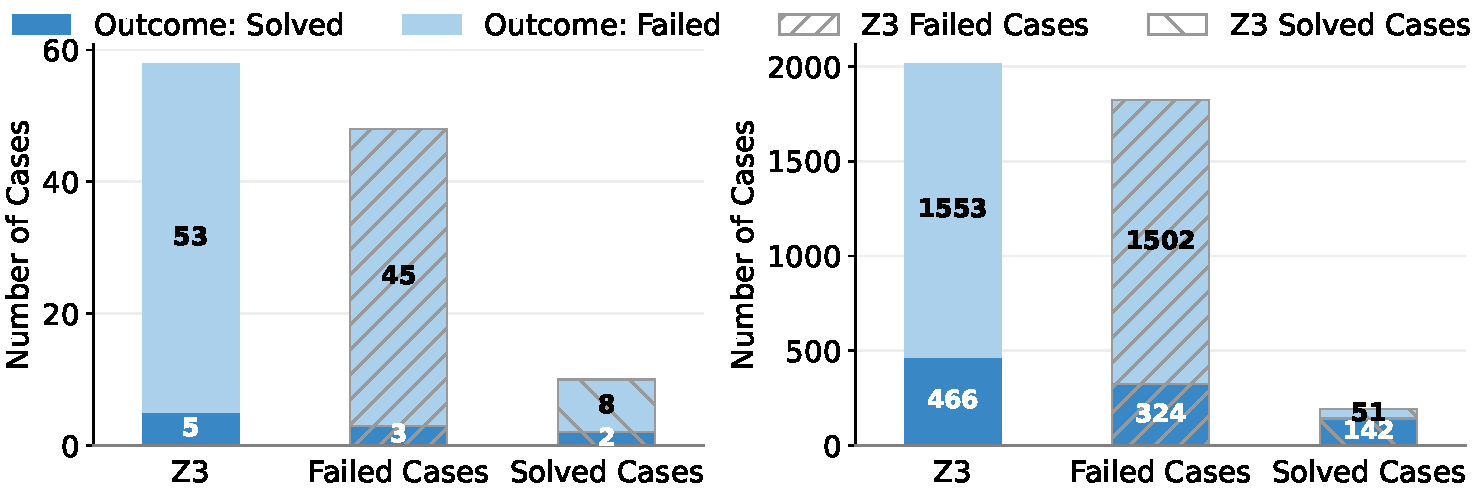
\includegraphics[width=0.9\textwidth]{pics/RQ2-scalability.pdf}
  \caption{Scalability on \SMTCOMP{} (\QFLIA{}, \QFNIA{})}
  \label{fig:RQ2-scalability}
\end{figure}

As shown in Figure~\ref{fig:RQ2-scalability}, our framework scales effectively to the diverse benchmarks from the SMT-COMP dataset, demonstrating its ability to generalize beyond program-derived constraints. Compared to the Z3 baseline, \tool{} achieves a +4.6\% improvement on \QFLIA{} and a +12.3\% improvement on \QFNIA{}. The performance gain is particularly pronounced on the challenging nonlinear integer arithmetic (\QFNIA{}) problems, where \tool{} successfully converts 324 instances that previously timed out (\texttt{unknown}) into solved (\texttt{sat}) cases. Furthermore, the framework preserves 74\% of the cases that the baseline Z3 could already solve, indicating that its benefits are largely complementary and not limited to simply accelerating already-solvable instances.

% \noindent\textbf{Answer to RQ1.} 
% \tool{} demonstrates comprehensive effectiveness. On the program-derived SMTimer benchmark, it delivers consistent, architecture-agnostic gains across all four diverse solvers evaluated, confirming its generalizability as a solver-independent framework. The performance increase is substantial; for instance, when paired with the widely-used Z3 solver, \tool{} increases the number of solved instances by \textbf{30.6\%} and provides a \textbf{2.6×} speedup on average for solved cases. Furthermore, \tool{} proves its ability to scale to more challenging problems on the SMT-COMP benchmarks, where it enables Z3 to solve \textbf{324} previously intractable nonlinear integer arithmetic instances.
\subsection{RQ2: Ablation Study of \tool{}}
\label{sec:rq2-ablation}

% Restructured RQ2 as comprehensive component analysis and model comparison, merging original RQ3 ablation studies with LLM model comparison experiments originally in RQ1, providing deeper internal mechanism analysis.

\subsubsection{LLM Ablation Study}
\begin{wraptable}{r}{0.7\textwidth}
\centering
\caption{Performance comparison across different language models on SMTimer dataset.}
\label{tab:llm-comparison}
\begin{tabular}{lccc}
\toprule
\textbf{Model Variant} & \textbf{Solved} & \textbf{Success Rate (\%)} & \textbf{Avg. Time (s)} \\
\midrule
\tool$_{\text{L3.1}}$ & \textbf{94} & \textbf{27.9} & \textbf{214} \\
\tool$_{\text{L3.3}}$ & 89 & 26.4 & 231 \\
\tool$_{\text{R1}}$ & 87 & 25.8 & 248 \\
\bottomrule
\end{tabular}
\end{wraptable}

% To understand the impact of the underlying language model, we evaluate three SOTA LLMs: LLaMA 3.1:70B, LLaMA 3.3:70B, and DeepSeek-R1:70B, denoted as \tool$_{\text{L3.1}}$, \tool$_{\text{L3.3}}$, and \tool$_{\text{R1}}$. The results, summarized in Table~\ref{tab:llm-comparison} and visualized in Figure~\ref{fig:llm-comparison}, reveal that the choice of LLM significantly affects performance, with \tool$_{\text{L3.1}}$ emerging as the most effective variant.

% Table~\ref{tab:llm-comparison} provides a quantitative summary, showing that \tool$_{\text{L3.1}}$ leads across all primary metrics: it achieves the highest solved count (\textbf{94}), the best success rate (\textbf{27.9\%}), and the lowest average solving time (\textbf{214s}). Figure~\ref{fig:llm-comparison} offers a deeper insight into the source of this success. It illustrates that \tool$_{\text{L3.1}}$'s superiority comes from a dual advantage: it not only solves more new instances (23) that the Z3 baseline failed on, but also demonstrates exceptional robustness by preserving 71 of the 72 (98.6\%) baseline cases. In contrast, the other variants exhibit lower preservation rates, indicating a trade-off that \tool$_{\text{L3.1}}$ successfully avoids.

% The superior performance of LLaMA 3.1:70B can be attributed to its training, which included a significant portion of code and other formal content, likely endowing it with a stronger capability for structured reasoning. In contrast, LLaMA 3.3:70B's fine-tuning appears to prioritize dialogue fluency, while DeepSeek-R1:70B shows a tendency to reframe the problem into a general reasoning narrative, both of which are less effective for the strict symbolic format of SMT solving. Based on its clear advantages in both solving new problems and preserving existing capabilities, we select \tool$_{\text{L3.1}}$ as the default configuration for all subsequent experiments.

% Reorganized RQ2 content order: first conduct LLM model comparison experiments, then component ablation studies, following logical sequence from model selection to component analysis.
To understand the impact of different \LLM{}s on overall performance, we evaluate three SOTA \LLM{}s: LLaMA 3.1:70B, LLaMA 3.3:70B, and DeepSeek-R1:70B, denoted as \tool$_{\text{L3.1}}$, \tool$_{\text{L3.3}}$, and \tool$_{\text{R1}}$ respectively. The results, summarized in Table~\ref{tab:llm-comparison} and visualized in Figure~\ref{fig:llm-comparison}, show that the choice of LLM significantly affects performance.
Table~\ref{tab:llm-comparison} provides a quantitative summary, showing that \tool$_{\text{L3.1}}$ leads across all primary metrics: it achieves the highest solved count (\textbf{94}), the best success rate (\textbf{27.9\%}), and the lowest average solving time (\textbf{214s}). This represents a substantial +30.6\% improvement over the Z3 baseline (72 solved) and consistently outperforms both \tool$_{\text{L3.3}}$ (89 solved) and \tool$_{\text{R1}}$ (87 solved). Besides，as shown in Figure~\ref{fig:llm-comparison}, \tool$_{\text{L3.1}}$ successfully resolves \textbf{71 of the 72} instances (a 98.6\% preservation rate) that the Z3 baseline could already handle, indicating its robustness. In contrast, \tool$_{\text{L3.3}}$ and \tool$_{\text{R1}}$ show lower preservation rates, solving 67 and 50 of the baseline cases, respectively. 
\begin{wrapfigure}{r}{0.48\textwidth}
    \centering
    \Description{A bar chart comparing the number of solved instances for different \LLM{}s variants of \tool, demonstrating model selection impact.}
    
\includegraphics[width=\linewidth]{pics/RQ1-effectiveness.pdf}
    \caption{LLM Model Comparison on SMTimer.}
    \label{fig:llm-effectiveness}
\end{wrapfigure}

The superior performance of LLaMA 3.1:70B can be attributed to its training data, which included a significant portion of code and other formal content. This appears to have endowed it with a stronger capability for structured reasoning, allowing it to generate concise and effective values that align well with the symbolic nature of SMT formulas. In contrast, while LLaMA 3.3:70B is built upon an improved version of the 3.1 model, its fine-tuning appears to prioritize dialogue fluency over strict formal reasoning. This tendency introduced unnecessary verbosity that reduced its efficiency on this highly structured task. Similarly, DeepSeek-R1:70B, despite its recognized strengths in general and mathematical reasoning, demonstrated a tendency to reframe the problem into a more general reasoning narrative rather than adhering closely to the strict symbolic format, resulting in less effective simplification. Based on its superior performance in this specialized domain, we select \tool$_{\text{L3.1}}$ as the default configuration for all subsequent experiments.

\subsubsection{Component Ablation Study}

\begin{wraptable}{r}{0.7\textwidth}
\centering
\caption{Component ablation study results on SMTimer dataset (Total=337 constraints).}
\label{tab:RQ3-ablation}
% use body font size
\begin{tabular}{lrrr}
\toprule
Method & Solved & Success Rate (\%) & Avg. Time (s) \\
\midrule
Random+Random & 62 & 18.4 & 416.8 \\
\LLM{} & 30 & 8.9 & 4.1 \\
Random+\LLM{} & 62 & 18.4 & 334.3 \\
\RL{}+Random & 84 & 24.9 & 429.0 \\
\RL{}+\LLM{} & \textbf{94} & \textbf{27.9} & \textbf{213.9} \\
\bottomrule
\end{tabular}
\end{wraptable}

% This is the introductory paragraph, which is good and remains unchanged.
To evaluate the contributions of each component, we conducted ablation studies comparing our full \RL{}+\LLM{} method against four baseline configurations: (i) Random+Random (both variable and value assignment are random), (ii) \LLM{} (\LLM{} handles both assignments without \RL{} guidance), (iii) Random+\LLM{} (random variable selection with \LLM{} value assignment), and (iv) \RL{}+Random (\RL{} variable selection with random values). 

% This is the REVISED analysis paragraph.
The results of this study, summarized in Table~\ref{tab:RQ3-ablation} and visualized in the performance profile plot in Figure~\ref{fig:RQ3-performance}, reveal a clear synergy between the two components. The full \RL{}+\LLM{} configuration significantly outperforms all baselines, achieving the highest solved count (94) and the fastest average time on solved instances (213.9s). The most critical insight comes from comparing the partial configurations: the \RL{}+Random variant (84 solved) dramatically outperforms the Random+\LLM{} variant (62 solved). This provides strong evidence that strategic variable selection, guided by the \RL{} agent, is the primary driver of performance, while semantically-guided value proposal, though beneficial, is secondary. Conversely, the \LLM{} approach performs poorly on its own (30 solved); its low average solving time (4.1s) indicates that it quickly solves trivial cases but lacks the strategic capability to handle more complex ones. 
The performance profile in Figure~\ref{fig:RQ3-performance} further corroborates these findings by illustrating the time-to-solution dynamics. The \RL{}+\LLM{} curve dominates all others, as it extends furthest to the right (solving the most instances) while remaining the lowest (solving them fastest). The plot also clearly shows that both variants relying on random variable selection (Random+Random and Random+\LLM{}) reach their limit early at 62 solved instances, reinforcing that variable selection is the key bottleneck. Conversely, the \LLM{} curve is the shortest and flattest, visually confirming that it only solves a small number of the easiest cases very quickly before failing on more complex problems.

\begin{figure}[t]

  \centering
  \Description{A performance profile plot comparing the solving time of \tool against other \LLM{}s.}
  
\includegraphics[width=0.9\textwidth]{pics/RQ3-performance.pdf}
  \caption{The performance of \tool on the SMTimer with different components.}
  \label{fig:RQ3-performance}
\end{figure}
\subsection{RQ3: Effectiveness of Selective Simplification}
\label{sec:rq3-routing}

While RQ1 and RQ2 demonstrate \tool{}'s effectiveness and component synergy, a practical question remains regarding its real-world viability. \tool{}'s AI-driven process, while powerful, introduces computational overhead compared to direct solving. Applying this expensive preprocessing to every constraint would be impractical in production environments, as many simpler problems can be solved more efficiently by the baseline solver alone. Therefore, an effective deployment strategy must selectively apply \tool{} only to those constraints identified as sufficiently complex to benefit from simplification.

To investigate such a selective simplification strategy, we simulate a production environment where the decision to apply \tool{} preprocessing is guided by predicted constraint complexity. We leverage the same \QFNIA{} benchmark established in our SMT-COMP evaluation, using the complete test set (10,043 constraints) with Z3 as the backend solver. The routing decision is driven by the time-bucket predictor from our pre-trained prediction models, configured with a threshold ($\geq 4$) that identifies approximately 0.8\% of constraints as candidates for \tool{} preprocessing.
We evaluate the selective simplification strategy by sending easy constraints to direct solving and hard ones to \tool{} according to the predictor. Effectiveness is measured by outcome counts and time efficiency.
Table~\ref{tab:routing-performance} presents a comprehensive comparison between direct solving and our selective simplification approach, demonstrating the time reduction benefits achieved through selective \tool application while maintaining solution quality across all satisfiability categories.
Compared to direct solving, the selective simplification approach reduces \texttt{sat} average time by 12.6\% (28.3s $\to$ 24.7s) and overall average by 11.9\% (36.6s $\to$ 32.2s), saving 43,988s in total and converting 81 \texttt{unknown} cases to \texttt{sat}. The efficiency gains are achieved by applying \tool{} to only 0.8\% of constraints, demonstrating strong performance improvements with minimal computational overhead. In practice, this selective simplification delivers tangible deployment benefits across satisfiability categories while maintaining scalability. 
\begin{table}[b]
\centering
\caption{Performance comparison between direct solving and selective simplification on \QFNIA{} test set (10,043 constraints)}
\label{tab:routing-performance}
% use body font size
\normalsize
\begin{tabular}{p{2.2cm}cccccr}
\toprule
\textbf{Strategy} & sat & unsat & unknown & \textbf{sat Avg.} & \textbf{Overall Avg.} & \textbf{Total Time} \\
 & \textbf{Count} & \textbf{Count} & \textbf{Count} & \textbf{Time (s)} & \textbf{Time (s)} & \textbf{(s)} \\
\midrule
Direct Solving & 6,711 & 792 & 2,540 & 28.3 & 36.6 & 367,374 \\
Selective Simplification & 6,792 & 792 & 2,459 & 24.7 & 32.2 & 323,386 \\
\bottomrule
\end{tabular}
\end{table}




% \subsection{Effectiveness of Selective \tool{} Application 2}
% \label{sec:rq3-routing}

% Our final research question addresses the practical viability of \tool{} in real-world settings. While the previous sections established its effectiveness on challenging problems, \tool{}'s AI-driven process introduces computational overhead. A key question for deployment is therefore whether this cost can be managed to achieve a net system-wide performance gain. To investigate this, we evaluate a selective application strategy where a complexity-guided router decides whether to send a constraint directly to the solver or to our \tool{} framework first.

% We simulate a production environment using the large \QFNIA{} test set (10,043 constraints) and Z3 as our representative backend solver. The routing decision is driven by our pre-trained time-bucket predictor, which is configured with a threshold ($\geq 4$) to identify and route only the most challenging cases---approximately 0.8\% of the total---to \tool{}. The effectiveness of this hybrid routing strategy, compared to a direct solving baseline, is measured by outcome counts and time efficiency, with the comprehensive results presented in Table~\ref{tab:routing-performance}.


% Compared to direct solving, the hybrid approach reduces \texttt{sat} average time by 12.6\% (28.3s $\to$ 24.7s) and overall average by 11.9\% (36.6s $\to$ 32.2s), saving 43,988s in total and converting 81 \texttt{unknown} cases to \texttt{sat}. The efficiency gains are achieved by routing only 0.8\% of constraints to \tool{}, demonstrating strong performance improvements with minimal computational overhead.

% \noindent\textbf{Answer to RQ3.} The intelligent routing system demonstrates practical deployment effectiveness by selectively applying \tool to only 0.8\% of constraints, yet delivers measurable system-wide improvements: converting 81 \texttt{unknown} cases to \texttt{sat}, reducing \texttt{sat} solving time by 12.6\%, and saving 12.2 hours of total computation time. This confirms that a guided approach can effectively manage the cost-benefit trade-off of advanced simplification, making \tool{} viable for production environments.




% For experimental consistency across research questions, RQ5 uses the same QF\_NIA dataset as RQ2, maintaining identical experimental conditions and enabling direct comparison of results. The complete dataset contains 10,043 constraints for testing the routing system performance, with the predictive models having been trained on separate training data that was excluded from this evaluation set. This ensures that the predictive models used in RQ5 are identical to those validated in RQ2, providing experimental consistency and reliability. Unless otherwise noted, across all research questions we train predictors on half of the data and evaluate on the other half. For the same dataset and solver, we reuse the same trained predictors. In RQ5, routing is driven by the time-bucket predictor with a threshold of $\geq 4$ to target hard cases while keeping the routed fraction low. We choose $\geq 4$ as a mid-range illustrative setting to demonstrate practicality rather than to optimize the threshold; nearby choices yield similar qualitative trends. This choice routes only a small fraction of cases ($\approx$0.8\%) while yielding measurable gains.

% We evaluate the hybrid routing system by sending easy constraints to direct solving and hard ones to \tool according to the two predictors (solvability and time bucket with threshold $\geq 4$). Effectiveness is measured by outcome counts and time efficiency.

% Table~\ref{tab:routing-performance} presents a comprehensive comparison between direct solving and our hybrid routing approach, demonstrating the time reduction benefits achieved through selective \tool application while maintaining solution quality across all satisfiability categories.
% Compared to direct solving, the hybrid approach reduces \texttt{sat} average time by 12.6\% (28.3s $\to$ 24.7s) and overall average by 11.9\% (36.6s $\to$ 32.2s), saving 43,988s in total and converting 81 \texttt{unknown} cases to \texttt{sat}. The efficiency gains are achieved by routing only 0.8\% of constraints to \tool, demonstrating strong performance improvements with minimal computational overhead. In practice, this selective routing delivers tangible deployment benefits across satisfiability categories while maintaining scalability.